\documentclass[DM,lsstdraft,STR,toc]{lsstdoc}
\input meta.tex

\begin{document}

\def\milestoneName{WISE Data Loaded in PDAC}
\def\milestoneId{LDM-503-1}
\def\product{LSST Science Platform}

\setDocCompact{true}

\title[\milestoneId{}~Test Report]{\milestoneId{} (\milestoneName{})~Test Report}
\setDocRef{\lsstDocType-\lsstDocNum}
\setDocDate{\vcsdate}
\setDocUpstreamLocation{\url{https://github.com/lsst/lsst-texmf/examples}}
\author{% `git log --pretty=%an | sort --key=2 | uniq` ?
  Gregory P. Dubois-Felsmann
}

% Most recent last
\setDocChangeRecord{
\addtohist{1}{2018-04-22}{Initial version.}{Dubois-Felsmann}

}

\setDocCurator{Gregory P. Dubois-Felsmann}
\setDocUpstreamLocation{\url{https://github.com/lsst-dm/\lsstDocType-\lsstDocNum}}
\setDocUpstreamVersion{\vcsrevision}


\setDocAbstract{
This is the test report for \milestoneId{} (\milestoneName{}), an LSST DM level 2 milestone pertaining to the \product{}, with tests performed according to LSP-00, Portal and API Aspect Deployment of a Wide-Area Dataset.
}

\maketitle

\section{Introduction}
\label{sect:intro}

\subsection{Objectives}
\label{sect:objectives}

The \milestoneId{} milestone calls for the principal WISE primary mission and NEOWISE first-year catalogs to be loaded into the LSP Integration Environment, also known as the Prototype Data Access Center.
The LSP-00 test specification, defined in LDM-540, was used to verify that the data were loaded and that the data service provided meets a subset of requirements for functionality of the API Aspect and the Portal Aspect of the Science Platform.

\subsection{Scope}
\label{sect:scope}

The LSP-00 test specification describes a comprehensive set of tests exploring the functionality of the Science Platform as applied to catalog and image data.
The following test cases were carried out as part of the verification of this milestone:

\begin{description}
\item[LSP-00-00]{Verification of the presence of the expected WISE data}
\item[LSP-00-05]{Demonstration of low-volume and/or indexed queries against the WISE data via API}
\item[LSP-00-10]{Demonstration of table-scan queries against the WISE data via API}
\item[LSP-00-15]{Execution of basic catalog queries in the Portal}
\item[LSP-00-20]{Operation of the UI for interaction with tabular data results}
\item[LSP-00-35]{Linkage of catalog query results to related catalog data}
\end{description}

The LSP-00-25 and LSP-00-30 test cases are not included in this report, as they address image data functionality and the WISE data load to PDAC in the end did not include the image data.
The decision to avoid loading the image data was taken when the time required to load the WISE catalog data turned out to be larger than originally expected, and also required unanticipated hardware upgrades.
In addition to the time required for loading the WISE image data, providing a useful image cutout service would have required developing an LSST-stack (\verb|afw|) camera model for WISE, and this was judged to be an effort with very limited benefit to DM development.
The key usefulness of the WISE data in the DM context is as a scientifically realistic scaling test for Qserv, requiring the handling of tens of billions of rows, so the priorities for the data loading were set accordingly.

The image-oriented test cases can be performed against the SDSS data previously loaded in the PDAC, and will be executed and documented separately.\footnote{As a user convenience, the Portal Aspect in PDAC does provide some limited access to WISE image data directly from IRSA, but as it does not use LSST interfaces to do so, it is not included in this test.}

The WISE catalog data to be loaded included the following tables:

\begin{itemize}

\item AllWISE Source Catalog: this catalog is comparable to the projected LSST \texttt{Object} table, arising from source detection performed on the coaddition of all the data from the pre-hibernation year of WISE operations, including the primary 4-band data as well as shorter periods of 3-band (W1,W2,W3) and 2-band (W1,W2) data taken after the exhaustion of the stored cryogen.

\item AllWISE Multi-Epoch Photometry (MEP) Table: roughly comparable to LSST \texttt{ForcedSource}, arising from forced photometry on every single-epoch image, based on the sources in the AllWISE Source Catalog.  
Differs from \texttt{ForcedSource} in that WISE takes all four band images at once, so every row in this table contains data from all four bands.

\item Single-Epoch Photometry tables from four eras of the mission, comparable to LSST \texttt{Source}.  
Similarly to the MEP Table, the WISE imaging model produces measurements in each available band in each row.  
As the W4 and then W3 bands were shut down as the spacecraft warmed up, their columns were dropped from the table, leading to an evolution of the schema with time.  
The four eras and the associated official table names are:
  \begin{itemize}
  \item All-Sky Single Exposure (L1b) Source Table, from the primary cold mission, with all four bands operating;
  \item 3-Band Cryo Single Exposure (L1b) Source Table, from the brief period when the spacecraft was still cold enough to collect W3, but not W4, data;
  \item Post-Cryo Single Exposure (L1b) Source Table, containing only W1 and W2 data, from the period following the primary mission when the cryogen was fully exhausted but operations were continued, after which the spacecraft was put into hibernation until 2013;
  \item NEOWISE-R Year 1 Single Exposure Source Table, from the first year of operations after the reactivation of the spacecraft, and containing only W1 and W2 data.
  \end{itemize}
\end{itemize}

The LSP-00 tests verified that these tables were present on the PDAC and exercised a variety of operations against them in the Portal and API Aspects.
The rest of this report covers the six test cases into which this work was divided.

\subsection{System Overview}
\label{sect:systemoverview}

The \product{} is the part of the LSST Data Management System which presents the LSST Data Products,
a user computational environment, and a set of tools for interacting with them, 
to LSST's science users.

The system under test is the initial deployment of the \product{} in the Prototype Data Access Center (PDAC),
an initial application of the NCSA-provided ``integration environment''.
In the tested version of the PDAC, 
elements of the database systems (including a Qserv prototype),
a partial deployment of the API Aspect data access Web services (DAX),
and an early version of the Science User Interface and Tools (SUIT) Portal were operated on a hardware cluster managed by NCSA.
The Notebook Aspect was not included in this deployment at all.

Software deployment was done essentially manually on the systems provided by NCSA,
in some cases by traditional software installation and in some using Docker containers,
but no Kubernetes layer was involved.

\subsection{Applicable Documents}
\label{sect:appdocs}

\begin{tabular}[htb]{l l}
% \citeds{LDM-294} & LSST DM Project Management Plan\\
% \citeds{LDM-503} & DM Test Plan\\
% \citeds{LDM-540} & \product{} Test Specification\\
LDM-294 & LSST DM Project Management Plan\\
LDM-503 & DM Test Plan\\
LDM-540 & \product{} Test Specification\\
\end{tabular}


\section{Personnel}
\label{sect:personnel}

All test cases were executed by Gregory Dubois-Felsmann (Caltech/IPAC).


\subsection{Summary Table}
\label{sect:summarytable}

\begin{longtable} {|p{0.2\textwidth}|p{0.2\textwidth}|p{0.6\textwidth}|}\hline
{\bf TEST CASE ID} & {\bf PASS/FAIL} & {\bf COMMENTS} \\\hline
LSP-00-00 & Pass & Refer to \S\ref{sect:detail-lsp-00-00}. \\\hline
LSP-00-05 & Pass & Refer to \S\ref{sect:detail-lsp-00-05}. \\\hline
LSP-00-10 & Pass & Refer to \S ref{sect:lsp-00-10}. \\\hline
LSP-00-15 & Pass & Refer to \S ref{sect:lsp-00-15}. \\\hline
LSP-00-20 & Pass & Refer to \S ref{sect:lsp-00-30}. \\\hline
LSP-00-35 & Pass & Refer to \S ref{sect:lsp-00-35}. \\\hline
\end{longtable}

\subsection{Overall Assessment}
\label{sect:overallassessment}

The test cases executed passed with a variety of minor issues relating to the details of the data import and features not fully implemented in this early version of the Science Platform.
Overall the test showed that it was possible to import a several $\times 10^8$ row dataset and access it usefully through Qserv and the Portal and API Aspects.

\subsection{Impact of Test Environment}
\label{sect:impact}

As noted above, the deployment of the database, API Aspect, and Portal Aspect components did not use Kubernetes and is not reflective of the planned final system.
This affected not only the management of the components but substantive technical aspects of their behavior;
in particular, in the Kubernetes deployment there will be ingress controllers and other components that affect the connections between components.

Furthermore, the external access control to the components was through a VPN rather than by means of LSP-level authentication and authorization,
and therefore most likely not reflective of parameters such the latency and throughput to be expected from the final system.

No tests of authorization and access control behaviors were performed.


\subsection{Recommended Improvements}
\label{sect:recommendations}

\begin{itemize}

\item{The current cone-search query size limits in the Portal are unreasonably small and Qserv would clearly support larger ones.}
\item{The PDAC TAP service does not support standard ADQL and required the use of Qserv-specific functions in order to exploit its performance successfully.}

\end{itemize}



\section{LSP-00-00: Verification of the presence of the expected WISE data}
\label{sect:detail-lsp-00-00}

The tests were performed primarily from an Apple laptop computer running OS X 10.11.6, wirelessly connected to the Internet and using the NCSA VPN at \texttt{vpn.illinois.edu}.
API Aspect queries were performed using a combination of the Python \texttt{requests} package and the \texttt{curl} command.
Notebooks were executed using Jupyter versions up through 5.4.1 and Python version 3.6.1.
The Portal was accessed using Safari 11.0.2.

\subsection{API Aspect tests}

The API Aspect tests made use of the "v0" \texttt{dbserv} service at 

\begin{center}
\texttt{http://lsst-qserv-dax01.ncsa.illinois.edu:5000/db/v0/tap/sync}.
\end{center}

This service accepts SQL queries, forwards them to Qserv for execution, and returns the results as JSON structures.
The open-source Python \emph{Requests} package\footnote{\texttt{http://github.com/requests/requests}} was used to perform the HTTP GET and POST operations required, and to parse the returned JSON structures into Python dictionaries.

\subsubsection{Table presence verification}
\label{sect:lsp-00-00-api-tables}

API Aspect \verb|dbserv| queries (\texttt{SHOW DATABASES} and \texttt{SHOW TABLES}) were used to establish the set of databases available, and within those databases, identify the WISE catalog tables of interest for the tests.

\begin{table}[h]
\centering
\begin{tabular}{p{0.4\textwidth} l l}
WISE catalog & PDAC database & PDAC table \\ \hline
AllWISE Source Catalog & \verb|wise_00| & \verb|allwise_p3as_psd| \\
AllWISE Multi-Epoch Photometry Table & \verb|wise_00| & \verb|allwise_p3as_mep| \\
All-Sky Single Exposure (L1b) Source Table & \verb|wise_4band_00| & \verb|allsky_4band_p1bs_psd| \\
3-Band Cryo Single Exposure (L1b) Source Table & \verb|wise_3band_00| & \verb|allsky_3band_p1bs_psd| \\
Post-Cryo Single Exposure (L1b) Source Table & \verb|wise_2band_00| & \verb|allsky_2band_p1bs_psd| \\
NEOWISE-R Year 1 Single Exposure Source Table & \verb|neowiser_yr1_00| & \verb|neowiser_yr1_p1bs_psd| \\
\end{tabular}
\caption{WISE tables as discovered through the PDAC DAX service}
\label{tab:wisetables}
\end{table}

\subsubsection{Table Schemas}
\label{sect:lsp-00-00-api-schema}

Schemas for the tables were obtained from \verb|DESCRIBE| queries on \verb|dbserv|.
The schemas were compared programmatically against those obtained from the 
appropriate IRSA program interface:

\begin{center}
\verb|https://irsa.ipac.caltech.edu/cgi-bin/Gator/nph-dd?mode=xml&catalog=|\textit{table}.
\end{center}

The results were parsed with the Python standard library class \verb|xml.etree.ElementTree|.
Comparison of the schemas was carried out in Python, without regard to the ordering of columns.
The following discrepancies were observed (details are preserved in the test notebook):

\begin{itemize}
\item The \verb|dec| column in each table was renamed to \verb|decl| to avoid a conflict with a reserved word in the Qserv implementation database.
\item The Qserv implementation adds special columns \verb|chunkId| and \verb|subChunkId| to each partitioned table.
\item The original column names in the \verb|wise_2band_00.allsky_2band_p1bs_psd| table all appear in the PDAC version converted to uppercase.
\item For some tables, The IRSA-published schemas via the program interface have additional columns compared to what is displayed in the IRSA Gator UI and, apparently, in addition to what was included in the export files used to load the PDAC Qserv.  
This was assessed to be irrelevant to the objectives of this test, and no serious effort was made to determine the reasons in time for this report, as this would have required IRSA staff time that was in short supply.
IRSA support tickets will be filed to ensure that the discrepancies are ultimately understood and, if possible and desirable, corrected.
The affected tables are:
  \begin{itemize}
  \item \verb|allwise_p3as_psd|: 36 columns appear in the IRSA program interface schema that do not appear in the PDAC table.
    Most of these are associated with a proper motion model fit.
  \item \verb|allsky_4band_p1bs_psd|: 20 columns appear in the IRSA program interface schema that do not appear in the PDAC table.
    16 of these seem to be intermediate data products of the photometry pipeline, including zero-point corrected PSF and aperture magnitudes and the zero points themselves.
  \item \verb|neowiser_yr1_p1bs_psd| (compared against the IRSA program interface for the ``live'' table \verb|neowiser_p1bs_psd|): 24 columns appear in the IRSA program interface schema that do not appear in the PDAC table.  
    These again appear to be a set of intermediate data products.
  \end{itemize}
\end{itemize}

\subsubsection{Row counts}
\label{sect:lsp-00-00-api-count}

Row counts were obtained from \verb|COUNT(*)| queries against all six tables.
These queries require accessing all chunks and subchunks in the Qserv partitioning and therefore resulted in table scans taking several minutes of wall clock time each.
The row counts and representative query durations are shown in Table \ref{tab:wisetablerows}.
The pattern of query times has not been fully understood; \verb|allwise_p3as_psd| is a notable outlier.
The row counts were compared to those advertised in the WISE documentation at IRSA.
They agree exactly except for the AllWISE Multi-Epoch Photometry Table, \verb|allwise_p3as_mep|, for which 42,759,337,365 rows are reported in the IRSA documentation, a difference of 761,630,509 or 1.8\%.
This discrepancy has not yet been understood.

\begin{table}[h]
\centering
\begin{tabular}{l r r}
PDAC WISE table & Rows & \texttt{COUNT(*) duration} \\ \hline
\verb|allwise_p3as_psd| & 747,634,026 & 798s \\
\verb|allwise_p3as_mep| & 41,997,706,856 & 1457s \\
\verb|allsky_4band_p1bs_psd| & 9,479,433,101 & 993s \\
\verb|allsky_3band_p1bs_psd| & 3,703,319,374 & 278s \\
\verb|allsky_2band_p1bs_psd| & 7,337,642,955 & 535s \\
\verb|neowiser_yr1_p1bs_psd| & 18,468,575,586 & 759s \\
\end{tabular}
\caption{Row counts in PDAC WISE tables, with durations of the associated \texttt{COUNT(*)} queries}
\label{tab:wisetablerows}
\end{table}

\subsection{Portal Aspect}
\label{sect:lsp-00-00-portal}

The Portal Aspect was accessed in order to verify the accessibility of the WISE catalog data.

This work covers step 6 of the LSP-00-00 test case procedure.

\subsubsection{Step 6a}

The front page of the Portal Aspect for this test was:

\begin{center}
\texttt{https://lsst-sui-proxy01.ncsa.illinois.edu/suit/}
\end{center}

\subsubsection{Step 6b}

The front page presents an ``LSST Data'' screen which offers the catalog data available for access, associated with three ``projects'': SDSS, AllWISE, and the WISE and NEOWISE single-epoch photometry.

The radio buttons under the project selector show the tables available for selection.
All six WISE tables covered by this test specification are available, as seen in the following screen shots.

\begin{figure}
  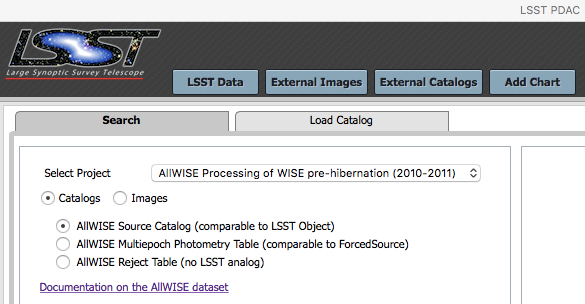
\includegraphics[width=\linewidth]{lsp-00-00/AllWISE-table-selection.png}
  \caption{AllWISE tables available for query in the Portal}
  \label{fig:portal-allwise-sel}
\end{figure}

\begin{figure}
  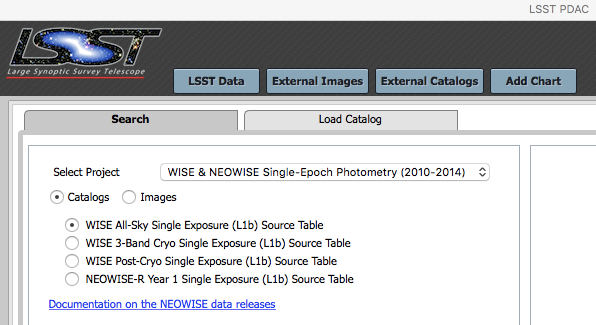
\includegraphics[width=\linewidth]{lsp-00-00/Single-Epoch-table-selection.png}
  \caption{WISE and NEOWISE single-epoch photometry tables available for query in the Portal}
  \label{fig:portal-singleepoch-sel}
\end{figure}

Given a selected table, the UI presents a selector for the type of search to be performed, offering a variety of options for spatial region searches including cone, ellipse, box, and polygon, as well as a multi-object cone search and a free-form all-sky search.
This UI element is shown in Figure \ref{fig:portal-search-methods} below.

\begin{figure}
  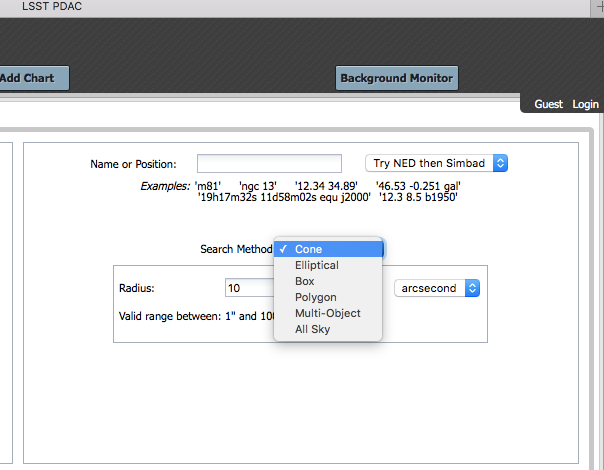
\includegraphics[width=\linewidth]{lsp-00-00/search-methods-pane.png}
  \caption{Search methods available for Portal queries on the WISE tables}
  \label{fig:portal-search-methods}
\end{figure}

\subsubsection{Step 6c}

The Portal also provides a UI element, shown in Figure \ref{fig:portal-schema-browser} displaying the entire table schema in a scrolling region, with, among other features, the ability to apply restrictions to any column for application in the query to be performed.
It was not a goal of this test to specifically validate the correct display of the schema, but some spot checks were performed and the results were as expected.
For instance, the schema display was observed to follow the expected pattern of whether W3- and W4-related were available in the selected table(s).
(The nature of the scrolling region provided for this selector inhibits easy capture of the entire content.
It would be useful for the final Portal to provide a UI element facilitating download of the entire schema.)
The schema anomalies reported in section \ref{sect:lsp-00-00-api-schema} above were also observed here, e.g., the uppercase conversion of the original column names in the \verb|allsky_2band_p1bs_psd| column.

Note that units and descriptions are not provided in the UI, though the layout anticipates them;
this is a consequence of the absence of a full \verb|metaserv| implementation at the time of the tests.

\begin{figure}
  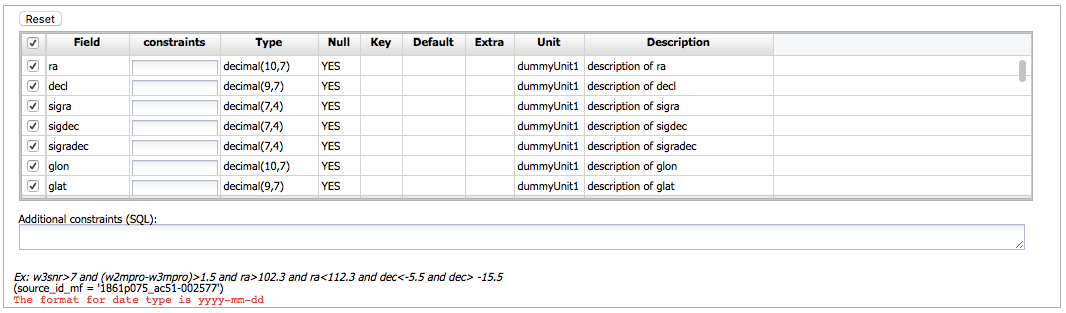
\includegraphics[width=\linewidth]{lsp-00-00/schema-browser.png}
  \caption{Schema browser and column-restriction API in the Portal, for WISE 3-band table}
  \label{fig:portal-schema-browser}
\end{figure}

The test specification calls for doing spot queries around (ra=0, dec=0); 
it turns out to be more useful to do them away from ra=0 so that in the default plots in the Portal plotting tool the points are not split across values just below 360 and just above 0.
(The values can be rescaled to (-180,180), of course, but this requires an extra step.)

100-arcsecond cone searches were successfully performed at (ra=1, dec=0) for all six tables.
The \verb|allsky_3band_p1bs_psd| search returned no rows, corresponding to this sky location not being included in the brief period of 3-band observation.
Screen shots are provided for \verb|allwise_p3as_psd| and \verb|neowiser_yr1_p1bs_psd|, and tabular results for all five non-empty queries are stored in the DMTR-52 repository.
Note the much larger number of sources for the NEOWISE-R single-epoch table query.

\begin{figure}
  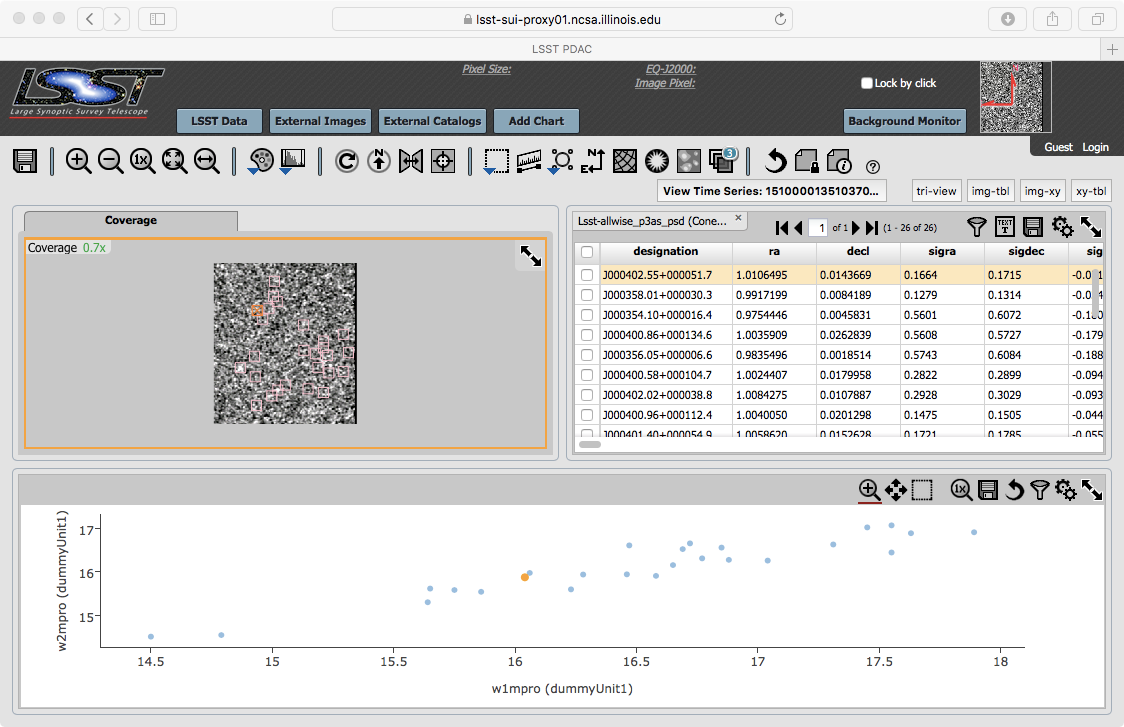
\includegraphics[width=\linewidth]{lsp-00-00/Portal-allwise_p3as_psd.png}
  \caption{Query at ra=1, dec=0 on the AllWISE Source Catalog}
  \label{fig:portal-query-allwise-psd}
\end{figure}

\begin{figure}
  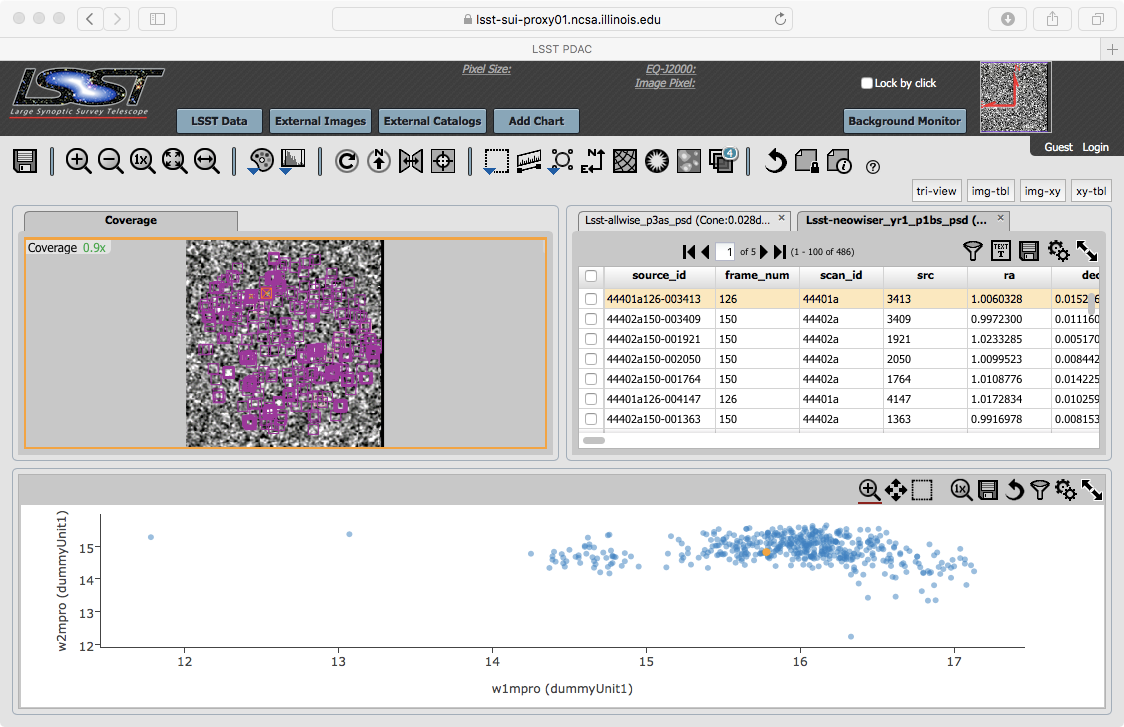
\includegraphics[width=\linewidth]{lsp-00-00/Portal-neowiser_yr1_p1bs_psd.png}
  \caption{Query at ra=1, dec=0 on the NEOWISE-R Year 1 Single-Epoch Source Catalog}
  \label{fig:portal-query-neowiser-psd}
\end{figure}


\section{LSP-00-05: Demonstration of low-volume and/or indexed queries against the WISE data via API}
\label{sect:detail-lsp-00-05}

The tests were performed primarily from an Apple laptop computer running OS X 10.11.6, wirelessly connected to the Internet and using the NCSA VPN at \texttt{vpn.illinois.edu}.
API Aspect queries were performed using a combination of the Python \texttt{requests} package and the \texttt{curl} command.
Notebooks were executed using Jupyter versions up through 5.4.1 and Python version 3.6.1.

\subsection{API Aspect tests}

This test case consisted only of API Aspect tests.

The API Aspect tests made use of the "v0" \texttt{dbserv} service at 

\begin{center}
\texttt{http://lsst-qserv-dax01.ncsa.illinois.edu:5000/db/v0/tap/sync},
\end{center}

as for LSP-00-00 above.

Comparison data was obtained from the IRSA TAP service at

\begin{center}
\texttt{https://irsa.ipac.caltech.edu/TAP/sync}.
\end{center}

This service accepts SQL queries, forwards them to Qserv for execution, and returns the results as JSON structures.
The open-source Python \emph{Requests} package\footnote{\texttt{http://github.com/requests/requests}} was used to perform the HTTP GET and POST operations required, and to parse the returned JSON structures into Python dictionaries.
The builtin Python \texttt{xml.etree.ElementTree} class was used to parse the VOTable data returned from the IRSA TAP service.

\subsubsection{Summary}

The tests successfully verified that the PDAC and IRSA services return the same data for small-diameter cone searches, 
down to floating point roundoff issues associated with the return of data as ASCII strings.

The cone search queries were performed in the Galactic plane near Galactic coordinates ( 30, 0 ),
expressed as ( \emph{ra} = 281.5, \emph{dec} = -2.6 ), with a radius of 100 arcseconds.
The radius was chosen to match the largest currently available radius for cone searches in the Portal UI 
(a relatively arbitrary number originally chosen based on IRSA experience with querying the MultiEpoch Photometry table).

In general the PDAC queries executed substantially more quickly than the IRSA ones.
IRSA queries on the tables tested took several times longer.
The IRSA times fluctuated more on repeated access, 
presumably because IRSA is an active community archive and has a fluctuating load of other queries.

The two TAP services do not accept the same language at this time.
DAX \texttt{dbserv} ``v0'' does not implement ADQL spatial query constructs, 
but does require the use of special Qserv UDFs to enable optimized spatial queries.
As a result, the spatial \texttt{WHERE} clauses look quite different.

\begin{table}[h]
\centering
\begin{tabular}{l l}
TAP Service & \texttt{WHERE} clause \\ \hline
PDAC \texttt{dbserv} & \verb|qserv_areaspec_circle(| \texttt{281.5, -2.6, 0.027777777777777776 )} \\
IRSA (ADQL) & \texttt{CONTAINS(POINT('J2000',ra,dec),CIRCLE('J2000',281.5,-2.6,0.027777777777777776))=1} \\
\end{tabular}
\caption{Comparison of PDAC and IRSA cone search query syntax}
\label{tab:conesyntax}
\end{table}

\subsubsection{Queries performed}

The cone-search queries returned the following results, with a range of elapsed times noted for repeating the query several times.

\begin{table}[h]
\centering
\begin{tabular}{p{0.5 \linewidth} p{0.1 \linewidth} p{0.1 \linewidth} p{0.12 \linewidth} p{0.12 \linewidth}}
Table & Unique Object Keys & Rows & PDAC elapsed time & IRSA elapsed time \\ \hline
``Object'' \verb|wise_00.allwise_p3as_psd| & 48 & 48 & 0.2 -- 0.6s & 1.4 -- 3.2s \\
``ForcedSource'' \verb|wise_00.allwise_p3as_mep| & 56 & 1377 & 0.8 -- 1.8s & 6.1 -- 6.6s \\
``Source'' \verb|wise_4band_00.allsky_4band_p1bs_psd| & 506 & 506 & 0.5 -- 0.6s & 1.6 -- 3.3s \\
\end{tabular}
\caption{Search results from small cone searches}
\label{tab:conesyntax}
\end{table}

All the sources found in the Object-like table were found in the ForcedSource-like table.
Note that the WISE data analysis includes forced photometry on lower-quality objects,
not just those in the main Object-like ``AllWISE Source Catalog'';
this is why there are more unique object keys in the ForcedSource-like table search result than in the Object-like searh result.

All the IDs were tested for exact equality, with no failures.
All queries retrieved \verb|ra|, \verb|decl|, and the WISE W1 and W1 magnitudes \verb|w1mpro| and \verb|w2mpro|.
The time-dependent queries also retrieved the MJD mid-point of the corresponding observations.
All these floating-point values were found to be equal to the limits of the round trip through the slightly different ASCII formats produced by the two services;
in general discrepancies occurred when the IRSA TAP service returned additional non-significant digits,
producing values like 4.3340000000000005.

\section{LSP-00-10: Demonstration of table-scan queries against the WISE data via API}
\label{sect:lsp-00-10}

\section{LSP-00-15: Execution of basic catalog queries in the Portal}
\label{sect:lsp-00-15}

\section{LSP-00-20: Operation of the UI for interaction with tabular data results}
\label{sect:lsp-00-20}

\section{LSP-00-35: Linkage of catalog query results to related catalog data}
\label{sect:lsp-00-35}


\end{document}
